\documentclass[devoir3.tex]{subfiles}

\begin{document}

\newcommand\hlight[1]{\tikz[overlay, remember picture,baseline=-\the\dimexpr\fontdimen22\textfont2\relax]\node[rectangle,fill=blue!50,rounded corners,fill opacity = 0.2,draw,thick,text opacity =1] {$#1$};}

\section*{Question 2}
Donnez toutes les étapes de l’algorithme de Floyd pour calculer le plus court chemin entre toutes les paires de noeuds du graphe de la figure \ref{fig:fig1}. Donnez la matrice obtenue à chaque itération.

\begin{figure}[H]
	\centering
	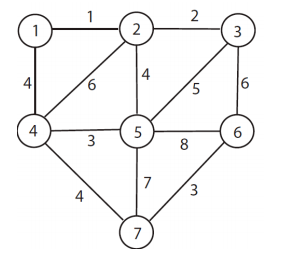
\includegraphics[width=8cm]{fig1}
	\caption{Graphe}
	\label{fig:fig1}
\end{figure}

La matrice D\textsubscript{0} qui suit est la matrice d'adjacence du graphe précédent:
\begin{align*}
	D\textsubscript{0} =
	\begin{bmatrix}
		0 	& 1 	  & \infty 	& 4 	  & \infty 	& \infty & \infty \\
		1 	& 0 	  & 2		& 6	  & 4		& \infty & \infty \\
		\infty  & 2 	  & 0 		& \infty & 5 		& 6 	  & \infty \\
		4 	& 6 	  & \infty   	& 0 	  & 3		& \infty & 4 \\
		\infty  & 4 	  & 5 		& 3 	  & 0 	 	& 8 	  & 7 \\
		\infty  & \infty & 6		& \infty & 8 		& 0 	  & 3 \\
		\infty 	& \infty & \infty 	& 4 	  & 7 		& 3 	 & 0
	\end{bmatrix}
\end{align*}

Pour la première itération de l'algorithme de Floyd, nous savons que la diagonale de 0, la colonne 1 et la ligne 1 seront semblables à celles de la matrice D\textsubscript{0}. Ensuite, pour construire le reste de la matrice nous utilisons la formule:
\begin{align*}
	D\textsubscript{k}[i,j] = Min(D\textsubscript{k-1}[i.j]. D\textsubscript{k-1}[i,k] + D\textsubscript{k-1}[k,j])
\end{align*}

Ce qui donne la matrice suivante, où les éléments [2,4] et [4,2] ont été modifiés:
\begin{align*}
	D\textsubscript{1} =
	\begin{bmatrix}
		0 	& 1 	  	& \infty 	& 4 	  	  & \infty 	& \infty & \infty \\
		1 	& 0 		& 2		& \hlight{5}	  & 4		& \infty & \infty \\
		\infty  & 2 		& 0 		& \infty 	  & 5 	  	& 6 	  & \infty \\
		4 	& \hlight{5}	& \infty   	& 0 	  	  & 3	  	& \infty & 4 \\
		\infty  & 4 	 	& 5 		& 3 	  	  & 0 	  	& 8 	  & 7 \\
		\infty  & \infty 	& 6		& \infty 	  & 8 	  	& 0 	  & 3 \\
		\infty 	& \infty 	& \infty 	& 4 	  	  & 7 	  	& 3 	 & 0
	\end{bmatrix}
\end{align*}

Puis, on répète jusqu'à ce qu'on est parcouru les 7 lignes/colonnes, ce qui donne les résultats suivants (tous les éléments sous-lignés ont été modifiés par rapport à la matrice précédente):
\begin{align*}
	D\textsubscript{2} =
	\begin{bmatrix}
		0 		& 1 	  	& \hlight{3} 	& 4 	  	  & \hlight{5}	& \infty & \infty \\
		1 		& 0 		& 2		& 5		  & 4		& \infty & \infty \\
		\hlight{3} 	& 2 		& 0 		& \hlight{7} 	  & 5 	  	& 6 	  & \infty \\
		4 		& 5		& \hlight{7}  	& 0 	  	  & 3	  	& \infty & 4 \\
		\hlight{5}  	& 4 	 	& 5 		& 3 	  	  & 0 	  	& 8 	  & 7 \\
		\infty  	& \infty 	& 6		& \infty 	  & 8 	  	& 0 	  & 3 \\
		\infty 		& \infty 	& \infty 	& 4 	  	  & 7 	  	& 3 	  & 0
	\end{bmatrix}
\end{align*}

\begin{align*}
	D\textsubscript{3} =
	\begin{bmatrix}
		0 		& 1 	  	& 3 		& 4 	  	  & 5		& \hlight{9} 	& \infty \\
		1 		& 0 		& 2		& 5		  & 4		& \hlight{8} 	& \infty \\
		3	 	& 2 		& 0 		& 7	 	  & 5 	  	& 6 		& \infty \\
		4 		& 5		& 7	  	& 0 	  	  & 3	  	& \hlight{13}	& 4 \\
		5  		& 4 	 	& 5 		& 3 	  	  & 0 	  	& 8 	 	& 7 \\
		\hlight{9}  	& \hlight{8} 	& 6		& \hlight{13}	  & 8 	  	& 0 	 	& 3 \\
		\infty 		& \infty 	& \infty 	& 4 	  	  & 7 	  	& 3 	 	& 0
	\end{bmatrix}
\end{align*}

\begin{align*}
	D\textsubscript{4} =
	\begin{bmatrix}
		0 		& 1 	  	& 3 		& 4 	  	  & 5		& 9	 	& \hlight{8} \\
		1 		& 0 		& 2		& 5		  & 4		& 8	 	& \hlight{9}  \\
		3	 	& 2 		& 0 		& 7	 	  & 5 	  	& 6 		& \hlight{11} \\
		4 		& 5		& 7	  	& 0 	  	  & 3	  	& 13		& 4 \\
		5  		& 4 	 	& 5 		& 3 	  	  & 0 	  	& 8 	 	& 7  \\
		9	 	& 8	 	& 6		& 13		  & 8 	  	& 0 	 	& 3   \\
		\hlight{8} 	& \hlight{9} 	& \hlight{11}	& 4 	  	  & 7 	  	& 3 	 	& 0
	\end{bmatrix}
\end{align*}

\begin{align*}
	D\textsubscript{5} =
	\begin{bmatrix}
		0 		& 1 	  	& 3 		& 4 	  	  & 5		& 9	 	& 8 \\
		1 		& 0 		& 2		& 5		  & 4		& 8	 	& 9  \\
		3	 	& 2 		& 0 		& 7	 	  & 5 	  	& 6 		& 11 \\
		4 		& 5		& 7	  	& 0 	  	  & 3	  	& \hlight{11}	& 4 \\
		5  		& 4 	 	& 5 		& 3 	  	  & 0 	  	& 8 	 	& 7  \\
		9	 	& 8	 	& 6		& \hlight{11}	  & 8 	  	& 0 	 	& 3   \\
		8 		& 9 		& 11		& 4 	  	  & 7 	  	& 3 	 	& 0
	\end{bmatrix}
\end{align*}

\begin{align*}
	D\textsubscript{6} =
	\begin{bmatrix}
		0 		& 1 	  	& 3 		& 4 	  	  & 5		& 9	 	& 8 \\
		1 		& 0 		& 2		& 5		  & 4		& 8	 	& 9  \\
		3	 	& 2 		& 0 		& 7	 	  & 5 	  	& 6 		& \hlight{9} \\
		4 		& 5		& 7	  	& 0 	  	  & 3	  	& 11		& 4 \\
		5  		& 4 	 	& 5 		& 3 	  	  & 0 	  	& 8 	 	& 7  \\
		9	 	& 8	 	& 6		& 11		  & 8 	  	& 0 	 	& 3   \\
		8 		& 9 		& \hlight{9}	& 4 	  	  & 7 	  	& 3 	 	& 0
	\end{bmatrix}
\end{align*}

\begin{align*}
	D\textsubscript{7} =
	\begin{bmatrix}
		0 		& 1 	  	& 3 		& 4 	  	  & 5		& 9	 	& 8 \\
		1 		& 0 		& 2		& 5		  & 4		& 8	 	& 9  \\
		3	 	& 2 		& 0 		& 7	 	  & 5 	  	& 6 		& 9   \\
		4 		& 5		& 7	  	& 0 	  	  & 3	  	& \hlight{7}	& 4 \\
		5  		& 4 	 	& 5 		& 3 	  	  & 0 	  	& 8 	 	& 7  \\
		9	 	& 8	 	& 6		& \hlight{7}	  & 8 	  	& 0 	 	& 3   \\
		8 		& 9 		& 9		& 4 	  	  & 7 	  	& 3 	 	& 0
	\end{bmatrix}
\end{align*}

La matrice résultante de l'algorithme de Floyd est donc:
\begin{align*}
	D\textsubscript{resultante} =
	\begin{bmatrix}
		0 		& 1 	  	& 3 		& 4 	  	  & 5		& 9	 	& 8 \\
		1 		& 0 		& 2		& 5		  & 4		& 8	 	& 9  \\
		3	 	& 2 		& 0 		& 7	 	  & 5 	  	& 6 		& 9   \\
		4 		& 5		& 7	  	& 0 	  	  & 3	  	& 7		& 4 \\
		5  		& 4 	 	& 5 		& 3 	  	  & 0 	  	& 8 	 	& 7  \\
		9	 	& 8	 	& 6		& 7		  & 8 	  	& 0 	 	& 3   \\
		8 		& 9 		& 9		& 4 	  	  & 7 	  	& 3 	 	& 0
	\end{bmatrix}
\end{align*}

\end{document}
